\documentclass[12pt]{article}
\usepackage{amsmath}
\usepackage{fancyhdr}
\usepackage{amssymb}
\usepackage{amsthm}
\usepackage{graphicx}
\usepackage{varioref}
\usepackage{verbatim} 
\usepackage{multicol}
\usepackage{enumerate}
\usepackage[normalem]{ulem}
%\usepackage[margin=1in]{geometry}
\usepackage{caption}
\usepackage{subcaption}
\usepackage[T1]{fontenc}
\usepackage[margin=1in]{geometry}
\usepackage{thm-restate}
\usepackage{enumitem}

%\usepackage{cite}
\usepackage{cite}



\usepackage{mathrsfs}

\usepackage{url}\urlstyle{same}
\usepackage{xspace}
\usepackage{thm-restate}

% Nicer font
\usepackage{mathpazo}


% Microtype
\usepackage{microtype}

% TikZ
\usepackage{tikz}
\usetikzlibrary{calc}
\usetikzlibrary{decorations.pathmorphing}
\usetikzlibrary{decorations.markings}
\usetikzlibrary{graphs,graphs.standard,quotes}

% Support eps figures
\usepackage{epstopdf}

% Hypertext package
\usepackage[colorlinks = true]{hyperref}
% Title and authors
%\hypersetup{
%  pdftitle = {},
%  pdfauthor = {}
%}
% Color definitions
\usepackage{xcolor}
\definecolor{darkred}  {rgb}{0.5,0,0}
\definecolor{darkblue} {rgb}{0,0,0.5}
\definecolor{darkgreen}{rgb}{0,0.5,0}
% Color links
\hypersetup{
  urlcolor   = blue,         % color of external links
  linkcolor  = darkblue,     % color of internal links
  citecolor  = darkgreen,    % color of links to bibliography
  filecolor  = darkred       % color of file links
}

% Clever references
\usepackage{cleveref}%[nameinlink]
\crefname{lemma}{Lemma}{Lemmas}
\crefname{proposition}{Proposition}{Propositions}
\crefname{definition}{Definition}{Definitions}
\crefname{theorem}{Theorem}{Theorems}
\crefname{conjecture}{Conjecture}{Conjectures}
\crefname{corollary}{Corollary}{Corollaries}
\crefname{section}{Section}{Sections}
%\crefname{property}{Property}{Properties}
\crefname{appendix}{Appendix}{Appendices}
\crefname{figure}{Fig.}{Figs.}
\crefname{equation}{Eq.}{Eqs.}
\crefname{table}{Table}{Tables}
\crefname{claim}{Claim}{Claims}
%\crefname{item}{Property}{Properties}

%%%%%%%%%%%%%%%%%%%%%%%%%
%  N E W T H E O R E M  %
%%%%%%%%%%%%%%%%%%%%%%%%%

\newtheorem{theorem}{Theorem}
\newtheorem{lemma}[theorem]{Lemma}
\newtheorem{proposition}[theorem]{Proposition}
\newtheorem{definition}[theorem]{Definition}
\newtheorem{corollary}[theorem]{Corollary}
\newtheorem{conjecture}[theorem]{Conjecture}
\newtheorem{property}[theorem]{Property}
\newtheorem*{conjecture*}{Conjecture}
\newtheorem*{problem}{Problem}
\newtheorem{claim}[theorem]{Claim}
\theoremstyle{definition}
\newtheorem*{remark}{Remark}
\newtheorem*{example}{Example}

\DeclareMathOperator{\E}{\mathrm{E}}		% expected value
\DeclareMathOperator{\pr}{\mathrm{P}}		% expected value
\DeclareMathOperator{\cov}{t_\textrm{cov}}  % cover time
\DeclareMathOperator{\hit}{t_{\textrm{hit}}}% hitting time

\newcommand{\todo}[1]{{\color{blue}{[{\bf TODO:} #1]}}}

\begin{document}


%+Title
\title{Cover Times of Random Walks}


\author{R. Teal Witter}

\date{\today}
%\date{\today}



\maketitle
%-Title

\abstract{abstract}

\newpage
\tableofcontents

\newpage
\section{Introduction and Background}

"white screen" problem
numerous applications
many mathematical tools

\subsection{Motivation}
universal travel sequences
graph connectivity
protocol testing

\subsection{Definitions}
We consider an undirected graph $G$ without self loops or multi-edges.
Let $V(G)$ be the set of vertices and let $E(G)$ be the set of edges on $G$.
Then $n$ is the number of vertices $|V(G)|$.
%Without loss of generality, we label the vertices $\{1, 2, 3, ..., n\}$.

We say $i\sim j$ for $i$ and $j$ in the vertex set $V(G)$ if $(i,j)$ in $E(G)$.
Let $c(i,j)$ be the non-negative weight of the edge between vertices $i$ and $j$.
If the graph is unweighted then $c(i,j) = 1$ if $i \sim j$.

Define the weight of vertex $i$ 
\begin{align}
c(i) &= \sum_{j:i \sim j} c(i,j). \nonumber
\end{align}

We consider a random walk $(X_t)$ on $G$.
Call $X_t$ the vertex that the walk is on at time $t$.
The random walker begins at vertex $X_0$.
At each step, the walker at vertex $i$ moves to neighboring vertex
$j$ with probability $\frac{c(i,j)}{c(i)}$.

Let $T_{j}$ be the number of steps until the first visit to $j$.
Formally,
\begin{align}
T_{j} &= \textrm{min} \left\{t : X_t = j \right\}. \nonumber
\end{align}
Let the hitting time $\hit$ be the maximum expected time between two vertices on $G$.
Formally, 
\begin{align}
\hit &= \max_{i,j \in V(G)} \E_i[T_j]. \nonumber
\end{align}
Note that $\E_i[T_j] = \E[T_j | X_0 = i]$.
Let the cover time $\cov$ be the expected time until all vertices have been
visited by the random walk $(X_t)$.
Formally,
\begin{align}
\cov &= \E [ \max_{j \in V(G)} T_j ]. \nonumber
\end{align}

\subsection{Outline}


\section{Cover Times of Structured Graphs}

\subsection{Small Example}
Always possible to calculate exactly but the number of equations grows exponentially
Special graph \cite{BH94} full cover time from vertex 1
In symmetric cases, we can calculate it
In other cases, we have to rely on bounds

\subsection{Complete Graph}
We call the graph with $n$ vertices and ${n \choose 2}$ edges the complete graph.

\begin{figure}[ht]
	\centering
	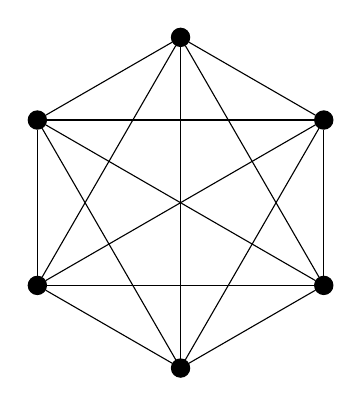
\begin{tikzpicture}[scale=.1]
	  \graph[circular placement, radius=3cm,
	         empty nodes, nodes={circle,draw,fill=black,scale=.7}] {
	    \foreach \x in {a,...,f} {
	      \foreach \y in {\x,...,f} {
	        \x -- \y;
	      };
	    };
	  };
	  \foreach \x [count=\idx from 0] in {a,...,f} {
	    \pgfmathparse{90 + \idx * (360 / 6)}
	    \node at (\pgfmathresult:4.4cm) {};
	  };
	\end{tikzpicture}
    \caption{The complete graph with six vertices (and ten edges).}\label{fig:complete}	
\end{figure}

Our goal is to find the expected number of steps until we have visited all
$n$ vertices in the complete graph.
Observe that the random walk can start at any vertex without loss of generality
because the graph is symmetric.
The strategy is to write the cover time $\cov$ in terms of the expected
value of more simple random variables.
Let $X_i$ be the random variable that represents the number of steps to go
from $i-1$ to $i$ unique vertices (excluding the current vertex).

We write the cover time in terms of $X_i$ and use linearity of expectation.
\begin{align}
\cov&= \E[X_1+X_2+X_3+...+X_{n+1}] = \sum_{i=1}^n \E[X_i] \nonumber
\end{align}

The random variable $X_i$ takes value $k$ when $k-1$ steps lead us to
already visited vertices and the $k^{th}$ step is to previously unvisited vertex.
It follows that $X_i$ is geometric with distribution
\begin{align}
\pr(X_i = k) = (1-p_i)^{k-1}p_i, \nonumber
\end{align}
where $p_i$ is the probability of moving to a previously unvisited vertex.
Then $\E[X_i] = \frac{1}{p_i}$. We now find $p_i$:
the probability that we go to a previously unvisited vertex is $\frac{n-i}{n-1}$.
This is because there are $n-i$ unvisited vertices and a total of $n-1$ adjacent vertices.
It follows that $\E[X_i] = \frac{n-1}{n-i}$.
Then
\begin{align}
\cov&=   \sum_{i=1}^n \frac{n-1}{n-i} \nonumber \\
&=  (n-1) \left(\frac{1}{n-1}+\frac{1}{n-2}+...+1\right). \nonumber
\end{align}

A natural interpretation of the cover time on a complete graph is 
the so-called coupon collecting problem.
There are $r$ different coupons that are randomly packaged in cereal boxes.
An avid fan buys a box of cereal every day.
We want to know how many days until the fan has collected each coupon.
The strategy is to think of every coupon as a vertex on the complete graph.
We then move from vertex to vertex with uniform probability.
The difference between the coupon collecting problem and the complete graph
is that we now have self-edges.
Before, we had to leave our current vertex at each step.
Now, we can stay in the same vertex (provided our collector found the same coupon
two days in a row).
We apply our approach to the complete graph and substitute the $r$ possible coupons
we can find for the $n-1$ vertices we could move to.
Then
\begin{align}
\cov&=  r \left(\frac{1}{r}+\frac{1}{r-1}+...+1\right). \nonumber
\end{align}

Another more subtle application of the cover time on a complete graph
is the cover time on an $n$-star.

\begin{figure}[ht]
	\centering
	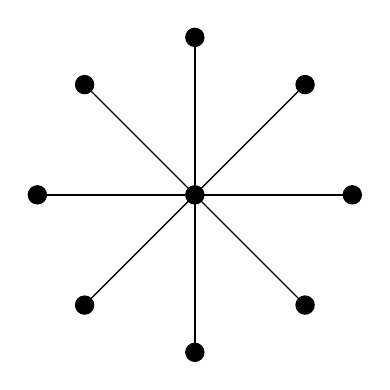
\begin{tikzpicture}[scale = 2]
	    \tikzstyle{vertex}=[draw, circle,fill=black, scale=.7]
	    \tikzstyle{edge}=[draw,line width = .5pt,-,black!100]
	    \node[vertex] (0) at (0,0) {};
	    \node[vertex] (1) at (1,0) {};
	    \node[vertex] (2) at (.7,-.7) {};
	    \node[vertex] (3) at (0,-1) {};
	    \node[vertex] (4) at (-.7,-.7) {};
	    \node[vertex] (5) at (-1,0) {};
	    \node[vertex] (6) at (-.7,.7) {};
	    \node[vertex] (7) at (0,1) {};
	    \node[vertex] (8) at (.7,.7) {};
	    \draw[edge] (1) -- (0);
	    \draw[edge] (2) -- (0);
	    \draw[edge] (3) -- (0);
	    \draw[edge] (4) -- (0);
	    \draw[edge] (5) -- (0);
	    \draw[edge] (6) -- (0);
	    \draw[edge] (7) -- (0);
	    \draw[edge] (8) -- (0);
	\end{tikzpicture}
	\caption{The nine-star.}\label{fig:n-star}
\end{figure}

An $n$-star is a graph with one central vertex and $n-1$ adjacent vertices each with a single
edge to the center.
A random walk begins at the central vertex and moves with uniform probability to
one of the $n-1$ adjacent vertices.
Whereas in the complete graph and coupon collecting problems we 
restarted in one step, a random walk on the $n$-star probabilistically restarts
in two steps: one step to each leaf and one step back.
We apply our approach to the complete graph and conclude that

\begin{align}
\cov&= 2(n-1) \left(\frac{1}{n-1}+\frac{1}{n-2}+...+1\right). \nonumber
\end{align}

\subsection{Simple Cycle}

A simple cycle is a connected graph where
each vertex has an edge to exactly two other vertices.
(\cref{fig:cycle} is an example.)

Our goal is to determine the cover time of a simple cycle.
However, we begin by considering the cover time of a subset
of the integers on the number line from $0$ to $N$.
We then use our analysis to build our way up to a simple cycle.

Consider a random walk on the finite linear graph.
(For the finite linear graph in \cref{fig:line}, note that $n=N+1$.)
From $X_t=i$, we move with equal probability to $i+1$
and $i-1$ until we reach either $0$ or $N$.

\begin{figure}[ht]
	\centering
	\begin{tikzpicture}
  		\pgfmathsetmacro{\N}{5}
		\tikzstyle{vertex}=[draw, circle,fill=black, scale=.7]
	    \tikzstyle{edge}=[draw,line width = .5pt,-,black!100]
		\tikzstyle{label}=[scale=.7]
		\draw[edge] (-\N,0) -- (\N,0);

		\node[label] (0) at (-\N,.5) {$0$};	
		\node[label] (N) at (\N,.5) {$N$};	
		\node[label] (0) at (-\N/5,.5) {$i$};

		\draw (-\N/5,0.1) -- (-\N/5,-0.1);
		\draw (\N,0.1) -- (\N,-0.1);
		\draw (-\N,0.1) -- (-\N,-0.1);

		\draw[edge] (-\N,0) -- (\N,0);
	\end{tikzpicture}
	\caption{A finite linear graph with a vertex at each integer from $0$ to $N$.}\label{fig:line}
\end{figure}

Call $e_i$ the expected number of steps until we reach either
end of our random walk from state $i$.
Our strategy is to write and solve a recurrence relation that
uses what we know about the random walk.
If $i=0,N$, we are already at the end point and $e_i=0$.
Otherwise, we take a step.
There's a half probability our step is to the right and
a half probability it is to the left.

\begin{align}
e_i &= 1 + \frac{1}{2} \left(e_{i+1}\right) + \frac{1}{2}\left(e_{i-1}\right) \nonumber \\
2 e_i &= 2 + e_{i+1} - e_{i-1} \nonumber \\
\left(e_{i+1} - e_i\right) &=\left( e_i - e_{i-1}\right) - 2 \nonumber
\end{align}

While the final line may look unnecessarily complicated,
notice that the structure of the equality lends itself to telescoping.

To solve the telescoping equations, notice that the walk is symmetric:
we could flip the walk over the vertical axis without changing $e_i$.
This makes sense because our intuition tells us that the only 
identifying feature of $i$ is its respective distances to the endpoints.
The logical conclusion is that $e_i=e_{N-i}$.
In particular, we have already seen that $e_0=e_N=0$ and it
naturally follows that $e_1=e_{N_1}$.
We use these observations to find $e_1$.

\begin{align}
\left(e_{2} - e_1\right) &= \left(e_1 - e_{0}\right) - 2 \nonumber \\
\left(e_{3} - e_2\right) &= \left(e_2 - e_{1}\right) - 2 = \left(e_1 - e_{0}\right) - 4\nonumber \\
\left(e_{4} - e_3\right) &= \left(e_3 - e_{2}\right) - 2 = \left(e_1 - e_{0}\right) - 6\nonumber \\
&\;\;\vdots \nonumber\\
\left(e_N - e_{N-1}\right) &= \left(e_1 - e_0\right) - 2 (N-1) \nonumber \\
\left(0 - e_1\right) &= \left(e_1 - 0\right) - 2 (N-1) \nonumber \\
e_1 &= N-1. \nonumber
\end{align}

(Note that the vertical dots denote inductive reasoning.)
We now know $e_1$.
However, our goal is to find the expected number of steps
from an arbitrary point $i$.
We use $e_1$ to find the general solution.

\begin{align}
e_2  &= e_1 + (e_1 - e_0) - 2 = 2 (N - 2) \nonumber\\
e_3  &= e_2 + (e_2 - e_1) - 2 = 2 \left[2 (N-2) \right] - (N-1) -2 = 3 (N - 3) \nonumber\\
&\;\;\vdots \nonumber\\
e_i &= i (N-i) \label{eq:line}
\end{align}

\cref{thm:line} follows from \cref{eq:line} and the observation that any
linear finite graph can be shifted so that the left end point
is at $0$ and the right end point is at $N$.

\begin{theorem}
The expected number of steps from a state to either end of a finite linear graph
is the product of the distances from that state to each end point.
\label{thm:line}
\end{theorem}

We now return to cover times.
Consider a random walk on a simple cycle as in \cref{fig:cycle}.
(Note that the starting vertex is arbitrary since the graph is symmetric.)
Think of $(X_t)$ as the walk on the number line (between $-n$ and $n$)
where $X_0 = 0$.
The cover time $\cov$ of the simple cycle is the expected number of steps 
until we visit $n$ distinct integers.

\begin{figure}[ht]
	\centering
	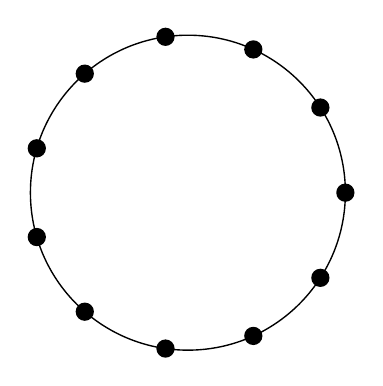
\begin{tikzpicture}
	\draw[line width=.5pt] circle (2cm);
	\foreach \a in {1,2,...,11} {
		\draw (\a*360/11: 2cm) node [circle, fill=black, scale=.7] (\a) {};
	}
	\end{tikzpicture}
	\caption{A cycle graph with $n=11$ vertices.}\label{fig:cycle}
\end{figure}

Let $\{a, a+1, \dots, b-1, b\}$ 
denote the set of vertices we have visited.
Since the walk is on a line, we can write $[a,b]$ for the range
of the walk where $a$ is the smallest 
and $b$ is the largest vertex we have visited.
Notice that if $a \leq -n$ or $b \geq n$, we have covered all $n$ vertices
on the simple cycle and conclude the random walk.

In a slight abuse of notation, let $T_k$ be the 
number of steps until we reach $k$ distinct vertices.
Formally, $T_k = \min{t: b-a+1 = k}$.
Then by telescoping,
\begin{align}
\cov &= \E[T_n] = \E[(T_2 - T_1) + (T_3 - T_2) + \dots + 
(T_k - T_{k-1}) + \dots + (T_n - T_{n-1})] \nonumber
\end{align}

At time $T_{k}$, we are either at integer $a$ or $b$.
Then $\E[T_{k+1}-T_{k}]$ is the expected time until we reach $a-1$ or $b+1$.
Notice that we can shift our end points to 0 and $b+1-(a-1) = b-a + 2 = k+1$.
The expected number of steps to either $a-1$ or $b+1$
is $1\dot (k+1-1) = k$ by \cref{thm:line}.

By linearity of expectation,
\begin{align}
\cov &=  (\E[T_2] - \E[T_1]) + \dots +
(\E[T_{k+1}] - \E[T_{k}]) + \dots + (\E[T_n] - \E[T_{n-1}]) \nonumber\\
&= 1 + 2 + \dots + k-1 + \dots + n-1  = \frac{1}{2}n(n-1). \nonumber
\end{align}

\subsection{Finite Linear Graph}
We have already seen a finite linear graph.
(For the finite linear graph in \cref{fig:line}, note that $n=N+1$).
\cref{thm:line} tells us the expected time from an arbitrary point to
one of the end points but we do not yet know the cover time.

Observe that the cover time is the earliest time that both end points 
have been visited.
We can use our earlier result to find the time to one of the end points
from an arbitrary position but we still need to find the expected time
from that end point to the other.

Consider $\E_i[T_N]$ the expected time to $N$ from vertex $i$.
We want to find $\E_0[T_N]$. By symmetry, $\E_0[T_N] = \E_N[T_0]$.



\section{Bounds}
\subsection{Matthews Method}


$\hit \leq \cov$

\begin{theorem}
Let $(X_t)$ be a random walk on a graph with $n$ vertices. Then \label{thm:matthews}
\end{theorem}
\begin{align}
\cov &\leq \hit \left(1 + \frac{1}{2} + \frac{1}{3} + ... + \frac{1}{n-1} \right). \nonumber
\end{align}

\begin{proof}
Without loss of generality, we may assume that the walk started at vertex $n$.
Let $\sigma$ be a uniform permutation of the unvisited $n-1$ vertices.
The strategy is to look for the vertices in order $\sigma$.
We call $\sigma_i$ the $i^{th}$ vertex we visit.
Let $T_k$ be the first time that vertices $\sigma_1, \sigma_2, ..., \sigma_k$
have all been visited.
For $1 \leq s \leq n-1$,
\begin{align}
\E_n[T_1 | \sigma_1 = s] = t_{n,s} \leq \hit \nonumber
\end{align}
\end{proof}

\subsection{Spanning Tree Argument}

\section{Distributional Aspects}
\subsection{Complete Graph}

\section{Electrical Networks}
\subsection{Definitions}
\subsection{Commute Times}
\subsection{Balanced Trees}

\section{Simulation}

\cite{AF14}
\cite{BH94}
\cite{Bo98}
\cite{DS84}
\cite{Du11}
\cite{Gr10}
\cite{LP17}

\newpage
\bibliography{mybib}{}
\bibliographystyle{plain}
\begin{comment}
\begin{thebibliography}{9}

\bibitem{AF14}
	Aldous, D. and J. Fill.
	2014.
	\textit{Reversible Markov Chains and Random Walks on Graphs}.

\bibitem{BH94}
	Blom, G., L. Holst and D. Sandell.
	\textit{Problems and Snapshots from the World of Probability},
	Springer Science \& Business Media, 1994.

\bibitem{Bo13}
	Bollobás, B.
	2013.
	\textit{Modern Graph Theory},
	Vol. 184,
	Springer Science \& Business Media.

\bibitem{DS84}
	Doyle, P. G. and J. L. Snell.
	1984.
	\textit{Random Walks and Electric Networks},
	Mathematical Association of America.
 
\bibitem{Gr10}
	Grimmett, G.
	2010.
	\textit{Probability on Graphs : Random Processes on Graphs and Lattices},
	Vol. 8,
	Cambridge University Press.

\bibitem{LP08}
	Levin, D. A. and Y. Peres.
	2017.
	\textit{Markov Chains and Mixing Times},
	Vol. 107,
	American Mathematical Society.

\end{thebibliography}
\end{comment}

\end{document}

